\documentclass[12pt,a4paper,notitlepage]{article}

\usepackage{./styles/plog1}

\addbibresource{plog1.bib}

\newcommand*{\foottitle}{Pente}
\newcommand*{\boardsize}[1]{#1\texttt{x}#1}

\title{
	\vspace{-2\baselineskip}
	
\includegraphics[scale=0.15]{feuplogo.jpg}\\
	{\Huge Pente}\\
	{\Large Game Overview, History and Rules}\\
	{\normalsize PLOG 2018}
}

\author{
	Bruno Dias da Costa Carvalho\hspace*{1.5em}\text{up201606517}
	\and
	Amadeu Prazeres Pereira\hspace*{1.5em}\text{up201605646} 
}

\begin{document}
\maketitle
\thispagestyle{empty}

\section{Overview and History}

\textbf{Pente} is an \textit{abstract strategy board game}, played usually by two players, in which the aim is to create an unbroken chain of five stones \emph{or} to capture ten of the enemy's stones.

It was created in 1977 by Gary Gabrel at the restaurant \textsl{Hideaway Pizza}, in Stillwater, Oklahoma, USA.\supercite{pente-wikipedia}
Customers waiting for their orders to arrive would play a variation of the game on checkerboard tablecloths.\supercite{pente-wikipedia}

Some variations allow for more than two independent players, and even teams, to play simultaneously. These require relaxing the winning conditions of the game to accommodate for the increased opposition --- namely requiring only a four-in-a-row for three or four players, and allowing mixed captures for teams.\supercite{pente-winning-moves}

The game has many variations for two player games -- all of which have a common ancestry in \textit{Gomoku}, which has a significantly simpler rule-set.
All variations of the game are played in the style of \textit{Go}, on the intersections of a traditional \boardsize{19} \emph{Go board} with black and white pieces called \emph{stones}. One player, \textsl{White}, uses the white stones, and the other, \textsl{Black}, uses the black stones. Once placed on the board, stones may not be moved, but may be removed from the board if \emph{captured}.

Introductory or speed games may be played on the smaller \boardsize{9} or \boardsize{13} boards, but the tighter space makes it very difficult to generate common patterns of play.

\section{Game Rules}

The game's precise rules vary considerably throughout variations and sources. As such, we'll first review the common base rules and then discuss a few variations.

\subsection{Base rules}

Let's recall there are two winning conditions, same for White and Black:

\begin{itemize}
	\large
	\item Form an unbroken chain of 5 or more consecutive friendly stones --- vertically, horizontally or diagonally.
	\item Capture a total of 10 enemy stones.
\end{itemize}

\begin{wrapfigure}[8]{r}[2em]{0.3\textwidth}
	\vspace*{-3\baselineskip}
	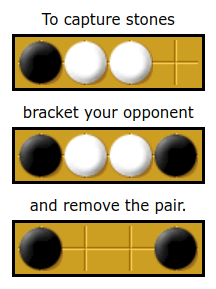
\includegraphics[scale=0.6]{capture.png}
	\caption{Capturing\supercite{pente-net} \label{fig:capture}}
\end{wrapfigure}

Unlike traditional \textit{Gomoku}, the chain may indeed have more than five consecutive stones.

\subsubsection{Captures}

Captures occur when two friendly adjacent stones (and only two) become bracketed by a pair of enemy stones, in a configuration depicted in \autoref{fig:capture}. Captures may arise in any direction.

\subsection{Variations}

Some sources add the following secondary rules.

\begin{itemize}
	\item White always plays first, in the center.\supercite{pente-renjunu, pente-wikipedia} This is unlike \textit{Renju} and \textit{Gomoku}.
	\item \textsl{Suicides} are not possible -- if a player places two adjacent friendly stones into a bracketed position --- forming the second panel of \autoref{fig:capture} --- his stones are not captured.\supercite{pente-renjunu,pente-org,pente-wikipedia,pente-winning-moves}
	\item Tournament Rule: The first player's second move is restricted -- it must be at least three intersections away from the center (that is, outside the middle \boardsize{5}).\supercite{pente-net,pente-org,pente-wikipedia,pente-winning-moves}
\end{itemize}

We'll be using these three rules hereafter.

Other sources do not specify starting player (or choose Black) and do not require the tournament rule, at least for casual play. 

Among variations we find: suicides allowed, called \textit{poofs} (\textit{Poof-Pente}); harsher Tournament Rule (\textit{G-Pente}, \textit{D-Pente}); 3-in-a-row captures (\textit{Keryo-Pente}), and others.\supercite{pente-org,pente-net}

\printbibliography

\end{document}